% LaTeX source for ``Python for Informatics: Exploring Information''
% Copyright (c)  2010-  Charles R. Severance, All Rights Reserved

\chapter{Listas}

\index{lista}
\index{tipo!list}


\section{Una lista es una secuencia}

Al igual que una cadena, una {\bf lista} es una secuencia de valores. En una cadena, los
valores son caracteres; en una lista, pueden ser de cualquier tipo. Los valores en las
listas reciben el nombre de {\bf elementos}, o a veces {\bf artículos}.

\index{elemento}
\index{secuencia}
\index{artículo}

Hay varios modos de crear una lista nueva; el más simple
consiste en encerrar los elementos entre corchetes (\verb"[" y \verb"]"):

\beforeverb
\begin{verbatim}
[10, 20, 30, 40]
['rana crujiente', 'vejiga de carnero', 'vómito de alondra']
\end{verbatim}
\afterverb
%
El primer ejemplo es una lista de cuatro enteros. El segundo es una lista
de tres cadenas. Los elementos en una lista no tienen por qué ser todos del mismo tipo.
La lista siguiente contiene una cadena, un flotante, un entero y
(¡ahí va!) otra lista:

\beforeverb
\begin{verbatim}
['spam', 2.0, 5, [10, 20]]
\end{verbatim}
\afterverb
%
Una lista dentro de otra se dice que está {\bf anidada}.

\index{anidada, lista}
\index{lista!anidada}

Una lista que no contiene elementos recibe el nombre
de lista vacía; se puede crear una simplemente
con unos corchetes vacíos, \verb"[]".

\index{vacía, lista}
\index{lista!vacía}

Como es lógico, puedes asignar listas de valores a variables:

\beforeverb
\begin{verbatim}
>>> quesos = ['Cheddar', 'Edam', 'Gouda']
>>> numeros = [17, 123]
>>> vacia = []
>>> print quesos, numeros, vacia
['Cheddar', 'Edam', 'Gouda'] [17, 123] []
\end{verbatim}
\afterverb
%

\index{asignación}

\section{Las listas son mutables}

\index{lista!elemento}
\index{accesso}
\index{índice}
\index{corchete, operador}
\index{operador!corchete}

La sintaxis para acceder a los elementos de una lista es la misma que
para acceder a los caracteres de una cadena---el operador corchete. La
expresión dentro de los corchetes especifica el índice. Recuerda que los
índices comienzan por 0:

\beforeverb
\begin{verbatim}
>>> print quesos[0]
Cheddar
\end{verbatim}
\afterverb
%
A diferencia de las cadenas, las listas son mutables (pueden mutar), porque puedes cambiar el orden
de los elementos o reasignar un elemento dentro de la lista.
Cuando el operador corchete aparece en el lado izquierdo de una asignación,
éste identifica el elemento de la lista que será asignado.

\index{mutabilidad}

\beforeverb
\begin{verbatim}
>>> numeros = [17, 123]
>>> numeros[1] = 5
>>> print numeros
[17, 5]
\end{verbatim}
\afterverb
%
El elemento de {\tt numeros} cuyo índice es uno, que
antes era 123, es ahora 5.

\index{índice!comienza en cero}
\index{cero, índice comienza en}

Puedes pensar en una lista como una relación entre índices y
elementos. Esta relación recibe el nombre de {\bf mapeo o direccionamiento}; cada índice
``dirige a'' uno de los elementos.


\index{elemento!asignación}
\index{asignación!elemento}

Los índices de una lista funcionan del mismo modo que los índices de una cadena:

\begin{itemize}

\item Cualquier expresión entera puede ser utilizada como índice.

\item Si se intenta leer o escribir un elemento que no existe,
se obtiene un {\tt IndexError}.

\index{exception!IndexError}
\index{IndexError}

\item Si un índice tiene un valor negativo, contará hacia atrás desde
el final de la lista.

\end{itemize}

\index{lista!índice}


\index{lista!pertenencia}
\index{pertenencia!lista}
\index{in, operador}
\index{operador!in}

El operador {\tt in} también funciona con las listas.

\beforeverb
\begin{verbatim}
>>> quesos = ['Cheddar', 'Edam', 'Gouda']
>>> 'Edam' in quesos
True
>>> 'Brie' in quesos
False
\end{verbatim}
\afterverb


\section{Recorrer una lista}
\index{lista!recorrido}
\index{recorrido!lista}
\index{for, bucle}
\index{bucle!for}
\index{sentencia!for}

El modo más habitual de recorrer los elementos de una lista es
con un bucle {\tt for}. La sintaxis es la misma que para las cadenas:

\beforeverb
\begin{verbatim}
for queso in quesos:
    print queso
\end{verbatim}
\afterverb
%
Esto funciona correctamente si sólo se necesita leer los elementos de la
lista. Pero si quieres escribir o modificar los elementos,
necesitarás los índices. Un modo habitual de hacerlo consiste en combinar
las funciones {\tt range} y {\tt len}:

\index{iteración!con índices}
\index{índice!iterando con}

\beforeverb
\begin{verbatim}
for i in range(len(numeros)):
    numeros[i] = numeros[i] * 2
\end{verbatim}
\afterverb
%
Este bucle recorre la lista y actualiza cada elemento. {\tt len}
devuelve el número de elementos de la lista. {\tt range} devuelve
una lista de índices desde 0 hasta $n-1$, donde $n$ es la longitud de
la lista. Cada vez que atravesamos el bucle, {\tt i} obtiene el índice
del elemento siguiente. La sentencia de asignación en el cuerpo usa
{\tt i} para leer el valor antiguo del elemento y asignarle el
valor nuevo.

\index{elemento, actualizar}
\index{actualizar!elemento}

Un bucle {\tt for} aplicado a una lista vacía no ejecuta nunca el código contenido en su cuerpo:

\beforeverb
\begin{verbatim}
for x in vacia:
    print 'Esto nunca ocurrirá.'
\end{verbatim}
\afterverb
%
A pesar de que una lista puede contener otra, la lista
anidada sólo cuenta como un único elemento. La longitud de esta lista
es cuatro:

\index{anidada, lista}
\index{lista!anidada}

\beforeverb
\begin{verbatim}
['spam', 1, ['Brie', 'Roquefort', 'Pol le Veq'], [1, 2, 3]]
\end{verbatim}
\afterverb



\section{Operaciones con listas}
\index{lista!operación}

El operador {\tt +} concatena listas:

\index{concatenación!lista}
\index{lista!concatenación}

\beforeverb
\begin{verbatim}
>>> a = [1, 2, 3]
>>> b = [4, 5, 6]
>>> c = a + b
>>> print c
[1, 2, 3, 4, 5, 6]
\end{verbatim}
\afterverb
%
De forma similar, el operador {\tt *} repite una lista el número especificado de veces:

\index{repeticion!lista}
\index{lista!repetición}

\beforeverb
\begin{verbatim}
>>> [0] * 4
[0, 0, 0, 0]
>>> [1, 2, 3] * 3
[1, 2, 3, 1, 2, 3, 1, 2, 3]
\end{verbatim}
\afterverb
%
El primer ejemplo repite {\tt [0]} cuatro veces. El segundo,
repite la lista {\tt [1, 2, 3]} tres veces.


\section{Rebanado de listas}

\index{rebanada!operador}
\index{operador!rebanada}
\index{índice!rebanada}
\index{lista!rebanada}
\index{rebanada!lista}
\index{slice!lista}
\index{lista!slice}

El operador de rebanada ({\tt slice}) también funciona en listas:

\beforeverb
\begin{verbatim}
>>> t = ['a', 'b', 'c', 'd', 'e', 'f']
>>> t[1:3]
['b', 'c']
>>> t[:4]
['a', 'b', 'c', 'd']
>>> t[3:]
['d', 'e', 'f']
\end{verbatim}
\afterverb
%
Si omites el primer índice, la rebanada comenzará al principio.
Si omites el segundo, la rebanada llegará hasta el final. De modo que
si omites ambos, la rebanada será una copia de la lista completa.

\index{lista!copiar}
\index{rebanada!copiar}
\index{copiar!rebanada}

\beforeverb
\begin{verbatim}
>>> t[:]
['a', 'b', 'c', 'd', 'e', 'f']
\end{verbatim}
\afterverb
%
Como las listas son mutables, a menudo resultará útil hacer una copia
antes de realizar operaciones que dupliquen elementos, los hagan rotar o mutilen
de algún modo esas listas.

\index{mutabilidad}

Un operador de rebanada en la parte izquierda de una asignación
puede modificar múltiples elementos:

\index{rebanada!actualizar}
\index{actualizar!rebanada}

\beforeverb
\begin{verbatim}
>>> t = ['a', 'b', 'c', 'd', 'e', 'f']
>>> t[1:3] = ['x', 'y']
>>> print t
['a', 'x', 'y', 'd', 'e', 'f']
\end{verbatim}
\afterverb
%

\section{Métodos de listas}

\index{lista!métodos}
\index{métodos!lista}

Python proporciona varios métodos que operan con listas. Por ejemplo,
{\tt append} añade un nuevo elemento al final de una lista:

\index{append, método}
\index{método!append}

\beforeverb
\begin{verbatim}
>>> t = ['a', 'b', 'c']
>>> t.append('d')
>>> print t
['a', 'b', 'c', 'd']
\end{verbatim}
\afterverb
%
{\tt extend} toma una lista como argumento y añade al final de la actual
todos sus elementos

\index{extend, método}
\index{método!extend}

\beforeverb
\begin{verbatim}
>>> t1 = ['a', 'b', 'c']
>>> t2 = ['d', 'e']
>>> t1.extend(t2)
>>> print t1
['a', 'b', 'c', 'd', 'e']
\end{verbatim}
\afterverb
%
En este ejemplo, {\tt t2} no se modifica.

{\tt sort} ordena los elementos de una lista de menor a mayor:

\index{sort, método}
\index{método!sort}

\beforeverb
\begin{verbatim}
>>> t = ['d', 'c', 'e', 'b', 'a']
>>> t.sort()
>>> print t
['a', 'b', 'c', 'd', 'e']
\end{verbatim}
\afterverb
%
La mayoría de los métodos de lista no devuelven nada; modifican la lista y devuelven {\tt None}.
Si escribes por accidente {\tt t = t.sort()}, seguro que te sientes defraudado
por el resultado.

\index{estéril, método}
\index{método!estéril}
\index{None, valor especial}
\index{valor especial!None}

\section{Borrado de elementos}

\index{borrado de elemento}
\index{borrado, elemento de lista}

Hay varias formas de borrar elementos de una lista. Si conoces
el índice del elemento que quieres eliminar, puedes usar
{\tt pop}:

\index{pop, método}
\index{método!pop}

\beforeverb
\begin{verbatim}
>>> t = ['a', 'b', 'c']
>>> x = t.pop(1)
>>> print t
['a', 'c']
>>> print x
b
\end{verbatim}
\afterverb
%
{\tt pop} modifica la lista y devuelve el elemento que ha sido eliminado.
Si no le proporcionas un índice, borra y devuelve el
último elemento.

Si no necesitas el valor eliminado, puedes usar el operador
{\tt del}:

\index{del, operador}
\index{operador!del}

\beforeverb
\begin{verbatim}
>>> t = ['a', 'b', 'c']
>>> del t[1]
>>> print t
['a', 'c']
\end{verbatim}
\afterverb
%

Si conoces el elemento que quieres eliminar (pero no su índice), puedes
usar {\tt remove}:

\index{remove, método}
\index{método!remove}

\beforeverb
\begin{verbatim}
>>> t = ['a', 'b', 'c']
>>> t.remove('b')
>>> print t
['a', 'c']
\end{verbatim}
\afterverb
%
El valor que devuelve {\tt remove} es {\tt None}.

\index{None, valor especial}
\index{valor especial!None}

Para eliminar más de un elemento, puedes usar {\tt del} con
un índice de rebanada:

\beforeverb
\begin{verbatim}
>>> t = ['a', 'b', 'c', 'd', 'e', 'f']
>>> del t[1:5]
>>> print t
['a', 'f']
\end{verbatim}
\afterverb
%
Como de costumbre, el método de rebanada selecciona todos los elementos hasta (pero
sin incluir) el segundo índice.

\section{Listas y funciones}

Hay varias funciones internas que pueden utilizarse en las listas
y que nos permiten buscar rápidamente a través de ellas
sin tener que escribir nuestros propios bucles:

\beforeverb
\begin{verbatim}
>>> nums = [3, 41, 12, 9, 74, 15]
>>> print len(nums)
6
>>> print max(nums)
74
>>> print min(nums)
3
>>> print sum(nums)
154
>>> print sum(nums)/len(nums)
25
\end{verbatim}
\afterverb
%
La función {\tt sum()} solamente funciona cuando los elementos de la lista son números.
Las otras funciones ({\tt max()}, {\tt len()}, etc.) funcionan también con listas
de cadenas y otros tipos que se puedan comparar.

Podemos reescribir un programa anterior que calculaba la media de
varios números introducidos por el usuario, usando ahora una lista.

Primero, el programa que calculaba la media sin usar listas:

\beforeverb
\begin{verbatim}
total = 0
contador = 0
while ( True ) :
    ent = raw_input('Introduzca un número: ')
    if ent == 'fin' : break
    valor = float(ent)
    total = total + valor
    contador = contador + 1

media = total / contador
print 'Media:', media
\end{verbatim}
\afterverb
%
En este programa, tenemos las variables {\tt contador} y {\tt total}
para almacenar la cantidad y el total actual de los números del usuario
según éste los va introduciendo.

Podemos simplemente guardar cada número que el usuario introduzca
y usar las funciones internas para calcular la suma y la cantidad
de números introducidos al final.

\beforeverb
\begin{verbatim}
listnum = list()
while ( True ) :
    ent = raw_input('Introduzca un número: ')
    if ent == 'fin' : break
    valor = float(ent)
    listnum.append(valor)

media = sum(listnum) / len(listnum)
print 'Media:', media
\end{verbatim}
\afterverb
%
Creamos una lista vacía antes de que el bucle comience, y luego cada vez
que tenemos un número lo añadimos a la lista. Al final del
programa, simplemente calculamos la suma de los números de la
lista y lo dividimos por la cantidad de números,
para obtener la media.

\section{Listas y cadenas}

\index{lista}
\index{cadena}
\index{secuencia}

Una cadena es una secuencia de caracteres y una lista es una secuencia
de valores, pero una lista de caracteres no es lo mismo que una
cadena. Para convertir desde una cadena a una lista de caracteres,
se puede usar la función {\tt list}:

\index{lista!función}
\index{función!list}

\beforeverb
\begin{verbatim}
>>> s = 'spam'
>>> t = list(s)
>>> print t
['s', 'p', 'a', 'm']
\end{verbatim}
\afterverb
%
Debido a que {\tt list} es el nombre de una función interna, debes
evitar usarla como nombre de variable. Yo también evito utilizar la letra {\tt l},
porque se parece mucho al número {\tt 1}. Por eso utilizo {\tt t}.

La función {\tt list} divide una cadena en letras individuales. Si
quieres dividir una cadena en palabras, puedes usar el método
{\tt split}:

\index{split, método}
\index{método!split}

\beforeverb
\begin{verbatim}
>>> s = 'suspirando por los fiordos'
>>> t = s.split()
>>> print t
['suspirando', 'por', 'los', 'fiordos']
>>> print t[2]
los
\end{verbatim}
\afterverb
%
Una vez hayas usado {\tt split} para dividir la cadena
en una lista de palabras, se puede utilizar el operador índice
(corchetes) para buscar una palabra concreta en la lista.

Puedes llamar a {\tt split} con
un argumento opcional llamado {\bf delimitador}, que
especifica qué caracteres se deben usar como delimitadores de palabras.
El ejemplo siguiente usa un guión como delimitador:

\index{opcional, argumento}
\index{argumento!opcional}
\index{delimitador}

\beforeverb
\begin{verbatim}
>>> s = 'spam-spam-spam'
>>> delimitador = '-'
>>> s.split(delimitador)
['spam', 'spam', 'spam']
\end{verbatim}
\afterverb
%
{\tt join} es la inversa de {\tt split}. Toma
una lista de cadenas y
concatena sus elementos. {\tt join} es un método de cadena,
de modo que debes invocarlo sobre el delimitador y pasarle
la lista como un parámetro:

\index{join, método}
\index{método!join}
\index{concatenación}

\beforeverb
\begin{verbatim}
>>> t = ['suspirando', 'por', 'los', 'fiordos']
>>> delimitador = ' '
>>> delimitador.join(t)
'suspirando por los fiordos'
\end{verbatim}
\afterverb
%
En caso de que el delimitador sea el carácter espacio,
entonces {\tt join} coloca un espacio entre las palabras. Para concatenar
cadenas sin espacios, puedes usar la cadena vacía,
\verb"''", como delimitador.

\index{cadena!vacía}


\section{Análisis de líneas}

Normalmente, cuando se está leyendo un archivo,
se deseará hacer con las líneas algo más que simplemente
imprimirlas completas en pantalla. A menudo se querrán encontrar
las ``líneas interesantes'' y luego {\bf parsear} (analizar) cada una de ellas
para buscar alguna \emph{parte} importante en su interior. ¿Qué ocurre si queremos
imprimir el día de la semana de aquellas líneas que comienzan por \mbox{``From ''?}

\beforeverb
\begin{alltt}
From stephen.marquard@uct.ac.za {\bf Sat} Jan  5 09:14:16 2008
\end{alltt}
\afterverb

El método {\tt split} es muy efectivo cuando nos enfrentamos con este
tipo de problemas.
Podemos escribir un pequeño programa que busque las líneas que
comiencen por ``From '', extraer las palabras de esas líneas con {\tt split},
y luego imprimir en pantalla la tercera palabra de cada una:

\beforeverb
\begin{verbatim}
manf = open('mbox-short.txt')
for linea in manf:
    linea = linea.rstrip()
    if not linea.startswith('From ') : continue
    palabras = linea.split()
    print palabras[2]
\end{verbatim}
\afterverb
%
Aquí utilizamos también la forma contraída de la sentencia
{\tt if}, de modo que colocamos el {\tt continue} en la
misma línea que el {\tt if}. Esta forma contraída
del {\tt if} opera igual que cuando el
{\tt continue} se coloca en la siguiente línea e indentado.

El programa produce la siguiente salida:

\beforeverb
\begin{verbatim}
Sat
Fri
Fri
Fri
    ...
\end{verbatim}
\afterverb
%
Más adelante, aprenderemos técnicas más sofisticadas para
seleccionar las líneas con las que vamos a trabajar y veremos cómo extraer
esas líneas para encontrar el fragmento exacto de información
que estamos buscando.

\section{Objetos y valores}

\index{objecto}
\index{valor}

Si ejecutamos estas sentencias de asignación:

\beforeverb
\begin{verbatim}
a = 'banana'
b = 'banana'
\end{verbatim}
\afterverb
%
sabemos que {\tt a} y {\tt b} se refieren ambas a una
cadena, pero no sabemos si se refieren a la
\emph{misma} cadena. Hay dos estados posibles:

\index{alias}

\beforefig
\centerline{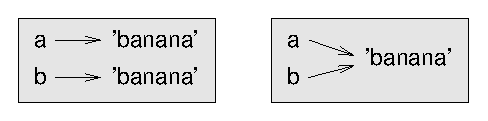
\includegraphics{figs2/list1.eps}}
\afterfig

En el primer caso, {\tt a} y {\tt b} se refieren a dos objetos diferentes que
tienen el mismo valor. En el segundo, se refieren al mismo
objeto.

\index{is, operador}
\index{operador!is}

Para comprobar si dos variables se refieren al mismo objeto, puedes
usar el operador {\tt is}.

\beforeverb
\begin{verbatim}
>>> a = 'banana'
>>> b = 'banana'
>>> a is b
True
\end{verbatim}
\afterverb
%
En este ejemplo, Python sólo crea un objeto cadena,
y tanto {\tt a} como {\tt b} se refieren a él.

Pero cuando creas dos listas, obtienes dos objetos:

\beforeverb
\begin{verbatim}
>>> a = [1, 2, 3]
>>> b = [1, 2, 3]
>>> a is b
False
\end{verbatim}
\afterverb
%

En este caso podríamos decir que las dos listas son {\bf equivalentes},
porque tienen los mismos elementos, pero no son {\bf idénticas}, porque
no son el mismo objeto. Si dos objetos son idénticos, también
son equivalentes, pero si son equivalentes, no necesariamente
son idénticos.

\index{equivalencia}
\index{identidad}

Hasta ahora, hemos estado usando ``objeto'' y ``valor''
de forma intercambiable, pero es más preciso decir que un objeto tiene
un valor. Si ejecutas {\tt a = [1,2,3]}, {\tt a} se refiere a un objeto
lista cuyo valor es una secuencia particular de elementos. Si otra
lista tiene los mismos elementos, podemos decir que tiene el mismo valor.

\index{objecto}
\index{valor}


\section{Alias}

\index{alias}
\index{referencia!alias}

Si {\tt a} se refiere a un objeto y asignas {\tt b = a},
entonces ambas variables se refieren al mismo objeto:

\beforeverb
\begin{verbatim}
>>> a = [1, 2, 3]
>>> b = a
>>> b is a
True
\end{verbatim}
\afterverb
%

La asociación de una variable con un objeto recibe el nombre de
{\bf referencia}. En este ejemplo, hay dos referencias para el mismo
objeto.

\index{referencia}

Un objeto con más de una referencia tiene más
de un nombre, de modo que decimos que el objeto tiene uno o varios {\bf alias}.

\index{mutabilidad}

Si el objeto con alias es mutable,
los cambios que se hagan en uno de los alias
afectarán al otro:

\beforeverb
\begin{verbatim}
>>> b[0] = 17
>>> print a
[17, 2, 3]
\end{verbatim}
\afterverb
%
A pesar de que este comportamiento puede resultar útil, es también propenso a errores. En general,
resulta más seguro evitar usar alias cuando se está trabajando con objetos
mutables.

\index{inmutabilidad}

Para objetos inmutables, como cadenas, usar alias no resulta tan
problemático. En este ejemplo:

\beforeverb
\begin{verbatim}
a = 'banana'
b = 'banana'
\end{verbatim}
\afterverb
%
casi nunca importa si {\tt a} y {\tt b} se refieren
a la misma cadena o no.


\section{Listas como argumentos}

\index{lista!como argumento}
\index{argumento}
\index{argumento!lista}
\index{referencia}
\index{parámetro}

Cuando se pasa una lista a una función, la función recibe una referencia
de esa lista.
Si la función modifica un parámetro de la lista, el código que la ha llamado también se verá afectado por el cambio.
Por ejemplo, \verb"borra_primer" elimina el primer elemento de una lista:

\beforeverb
\begin{verbatim}
def borra_primer(t):
    del t[0]
\end{verbatim}
\afterverb
%
Y aquí vemos el modo lo hemos usado:

\beforeverb
\begin{verbatim}
>>> letras = ['a', 'b', 'c']
>>> borra_primer(letras)
>>> print letras
['b', 'c']
\end{verbatim}
\afterverb
%
El parámetro {\tt t} y la variable {\tt letras} son
alias para el mismo objeto.

Resulta importante distinguir entre las operaciones que
modifican listas y las operaciones que crean listas nuevas.
Por ejemplo, el método {\tt append} modifica una lista, pero el
operador {\tt +} crea una lista nueva:

\index{append, método}
\index{método!append}
\index{lista!concatenación}
\index{concatenación!lista}

\beforeverb
\begin{verbatim}
>>> t1 = [1, 2]
>>> t2 = t1.append(3)
>>> print t1
[1, 2, 3]
>>> print t2
None

>>> t3 = t1 + [3]
>>> print t3
[1, 2, 3]
>>> t2 is t3
False
\end{verbatim}
\afterverb

Esta diferencia es importante cuando se escriben funciones que
se supone que modificarán listas. Por ejemplo, esta función
\emph{no} borra el primer elemento de una lista:

\beforeverb
\begin{verbatim}
def no_borra_primer(t):
    t = t[1:]              # ¡INCORRECTO!
\end{verbatim}
\afterverb

El operador de rebanada crea una lista nueva y la asignación
hace que {\tt t} se refiera a ella, pero ninguno de ellos tiene ningún efecto
sobre la lista que se ha pasado como argumento.

\index{rebanada!operador}
\index{operador!rebanada}

Una alternativa consiste en escribir una función que cree y
retorne una lista nueva. Por ejemplo,
{\tt cola} devuelve todos los elementos de la lista
excepto el primero:

\beforeverb
\begin{verbatim}
def cola(t):
    return t[1:]
\end{verbatim}
\afterverb
%
Esta función deja la lista original sin modificar.
Aquí está el modo como se usa:

\beforeverb
\begin{verbatim}
>>> letras = ['a', 'b', 'c']
>>> resto = cola(letras)
>>> print resto
['b', 'c']
\end{verbatim}
\afterverb


\begin{ex}

Escribe una función llamada {\tt recorta}, que tome una lista, la
modifique, eliminando los elementos primero y último, y devuelva {\tt None}.

Después escribe una función llamada {\tt centro}, que tome una lista y
devuelva otra que contenga todos los elementos de la original,
menos el primero y el último.

\end{ex}


\section{Depuración}
\index{depuración}

El uso descuidado de las listas (y otros objetos mutables)
puede ocasionar largas horas de depuración. He aquí algunas
trampas comunes y los modos de evitarlas:

\begin{enumerate}

\item No olvides que la mayoría de los métodos de las listas modifican el argumento y
devuelven {\tt None}. Esto es lo opuesto a lo que hacen los métodos de cadena,
que devuelven una cadena nueva y dejan la original inalterada.

Si estás acostumbrado a escribir código con cadenas como éste:

\beforeverb
\begin{verbatim}
palabra = palabra.strip()
\end{verbatim}
\afterverb

Resulta tentador escribir código con listas como éste:

\beforeverb
\begin{verbatim}
t = t.sort()           # ¡INCORRECTO!
\end{verbatim}
\afterverb

\index{sort, método}
\index{método!sort}

Como {\tt sort} devuelve {\tt None}, la operación
siguiente que realices con {\tt t} es probable que falle.

Antes de usar métodos de lista y operadores, deberías leer la
documentación con cuidado y luego probarlos en modo interactivo. Los
métodos y operadores que comparten listas con otras secuencias (como
cadenas) están documentados en
\url{https://docs.python.org/2/library/stdtypes.html#string-methods}.
Los métodos y operadores que sólo se pueden aplicar a secuencias mutables
están documentados en
\url{https://docs.python.org/2/library/stdtypes.html#mutable-sequence-types}.


\item Elige un estilo y ajústate a él.
\index{estilo}

Parte del problema con las listas es que hay demasiados
modos de hacer las cosas. Por ejemplo, para eliminar un elemento de
una lista, se puede usar {\tt pop}, {\tt remove}, {\tt del},
o incluso una asignación de rebanada ({\tt slice}).

Para añadir un elemento, se puede usar el método {\tt append} o
el operador {\tt +}. Pero no olvides que esto es correcto:

\beforeverb
\begin{verbatim}
t.append(x)
t = t + [x]
\end{verbatim}
\afterverb

Mientras que esto es incorrecto:

\beforeverb
\begin{verbatim}
t.append([x])          # ¡INCORRECTO!
t = t.append(x)        # ¡INCORRECTO!
t + [x]                # ¡INCORRECTO!
t = t + x              # ¡INCORRECTO!
\end{verbatim}
\afterverb

Prueba cada uno de estos ejemplos en modo interactivo para asegurarte
de que comprendes lo que hacen. Fíjate que sólo el último
causa un error en tiempo de ejecución; los otros tres son correctos sintácticamente, pero
hacen las cosas mal.


\item Haz copias para evitar los alias.

\index{alias!copiar para evitar}
\index{copiar!para evitar alias}

Si quieres usar un método como {\tt sort}, que modifica
el argumento, pero necesitas también mantener la lista original,
puedes hacer una copia.

\beforeverb
\begin{verbatim}
orig = t[:]
t.sort()
\end{verbatim}
\afterverb

En este ejemplo, puedes usar también la función interna {\tt sorted},
que devuelve una nueva lista ordenada, y deja la original sin modificar.
Pero en ese caso, ¡recuerda no utilizar {\tt sorted} como nombre de
variable!

\item Listas, {\tt split} y ficheros

Cuando leemos y analizamos ficheros, hay muchas oportunidades
de encontrar entradas que pueden hacer fallar nuestro programa, de modo que
es una buena idea recurrir al uso del patrón {\bf guardián} cuando
estemos escribiendo programas que lean a través de un archivo
y busquen ``una aguja en el pajar''.

Vamos a revisar el programa anterior que buscaba el día de la semana
en las líneas ``from'' de nuestro archivo:

\beforeverb
\begin{alltt}
From stephen.marquard@uct.ac.za {\bf Sat} Jan  5 09:14:16 2008
\end{alltt}
\afterverb

Dado que estamos partiendo esta línea en palabras, podemos apañarnos
con el uso de {\tt startswith} y simplemente revisar la
primera palabra de la línea para determinar si estamos interesados
en ella o no. Podemos usar {\tt continue} para saltar aquellas
líneas que no tengan ``From'' como primera palabra, como hacemos
a continuación:

\beforeverb
\begin{verbatim}
manf = open('mbox-short.txt')
for linea in manf:
    palabras = linea.split()
    if palabras[0] != 'From' : continue
    print palabras[2]
\end{verbatim}
\afterverb
%
Esto parece mucho más sencillo y ni siquiera tenemos que usar el
{\tt rstrip} para eliminar los saltos de línea al final de cada línea.
Pero, ¿es mejor hacerlo así?

\beforeverb
\begin{verbatim}
python search8.py 
Sat
Traceback (most recent call last):
  File "search8.py", line 5, in <module>
    if palabras[0] != 'From' : continue
IndexError: list index out of range
\end{verbatim}
\afterverb
%
Parece funcionar, y podemos ver el día extraído de la primera línea
(Sat), pero luego el programa falla con un error y su traceback correspondiente.
¿Qué es lo que ha ido mal? ¿Qué desastroso dato ha provocado que nuestro elegante,
ingenioso, y muy Pythónico programa haya fallado?

Puedes revisarlo durante largo rato y romperte la cabeza
con él, o pedir ayuda a alguien, pero el enfoque más
rápido e inteligente consiste en añadir una sentencia {\tt print}. El mejor lugar
para situarla es justo antes de la línea en la que
falla el programa, e imprimir el dato que parecer ser el causante
del error.

Ese diseño puede generar un montón de líneas en la salida, pero
al menos tendrás inmediatamente a mano alguna pista acerca
del problema. De modo que imprimiremos la variable
{\tt palabras} justo antes de la línea cinco. Incluso
añadiremos el prefijo ``Debug:'' a la línea, para que
podamos mantener nuestra salida normal separada de la de depuración:

\beforeverb
\begin{verbatim}
for linea in manf:
    palabras = linea.split()
    print 'Debug:', palabras
    if palabras[0] != 'From' : continue
    print palabras[2]
\end{verbatim}
\afterverb
%
Cuando hacemos funcionar el programa, un montón de texto de salida
desplaza la pantalla hasta arriba. Al final veremos nuestra salida
de depuración y el traceback, de modo que podremos saber qué
ha ocurrido justo antes de producirse el error.

\beforeverb
\begin{verbatim}
Debug: ['X-DSPAM-Confidence:', '0.8475']
Debug: ['X-DSPAM-Probability:', '0.0000']
Debug: []
Traceback (most recent call last):
  File "search9.py", line 6, in <module>
    if palabras[0] != 'From' : continue
IndexError: list index out of range
\end{verbatim}
\afterverb
%
Cada línea de depuración está imprimiendo la lista de palabras que obtenemos
cuando {\tt dividimos} la línea en palabras. Cuando el programa falla,
la lista de palabras está vacía \verb"[]". Si abrimos el archivo en un
editor de texto y observamos su contenido, en ese punto podremos observar
lo siguiente:

\beforeverb
\begin{verbatim}
X-DSPAM-Result: Innocent
X-DSPAM-Processed: Sat Jan  5 09:14:16 2008
X-DSPAM-Confidence: 0.8475
X-DSPAM-Probability: 0.0000

Details: http://source.sakaiproject.org/viewsvn/?view=rev&rev=39772
\end{verbatim}
\afterverb
%
¡El error se produce cuando nuestro programa encuentra una línea en blanco! Por supuesto,
hay ``cero palabras'' en una línea en blanco. ¿Por qué no hemos pensado en eso
cuando estábamos escribiendo el código? Cuando el código busca la primera
palabra (\verb"palabras[0]"), para comprobar si coincide con ``From'',
obtenemos un error ``index out of range'' (índice fuera de rango).

Por supuesto, éste es el lugar perfecto para añadir un código {\bf guardián},
que impida revisar la primera palabra si resulta que no existe primera palabra.
Hay muchos modos de proteger este código; vamos a optar por
comprobar el número de palabras que tenemos antes de mirar cuál es la primera palabra:

\beforeverb
\begin{verbatim}
manf = open('mbox-short.txt')
contador= 0
for linea in manf:
    palabras = linea.split()
    # print 'Debug:', palabras
    if len(palabras) == 0 : continue
    if palabras[0] != 'From' : continue
    print palabras[2]
\end{verbatim}
\afterverb
%
Primero hemos comentado la sentencia print de depuración en lugar de eliminarla,
para que si nuestra modificación falla podamos depurarlo de nuevo. Después, hemos añadido
una sentencia guardián que comprueba si tenemos cero palabras, y si es así,
usamos {\tt continue} para saltar a la siguiente línea del archivo. 

Podemos pensar en las dos sentencias {\tt continue} como ayudas para seleccionar
el conjunto de líneas que nos resultan ``interesantes'' y que querremos
procesar un poco más. Una línea que no tiene palabras resulta ``irrelevante'' para
nosotros, de modo que saltamos a la siguiente. Una línea que no tiene ``From''
como primera palabra también resulta irrelevante para nosotros, así que también la saltaremos.

El programa modificado funciona correctamente, así que tal vez sea correcto. Nuestra
sentencia guardián nos asegura que {\tt palabras[0]} no fallará nunca,
pero tal vez eso no sea suficiente. Cuando estamos programando, siempre debemos
estar pensando: ``¿Qué podría salir mal?''

\begin{ex}

Averigua qué línea del programa anterior aún no está suficientemente protegida.
Intenta construir un archivo de texto que provoque que el programa falle,
luego modifica el programa para que esa línea quede protegida adecuadamente, y
pruébalo para asegurarte de que es capaz de manejar tu nuevo archivo de texto.

\end{ex}

\begin{ex}
Reescribe el código guardián en el ejemplo de arriba para que no use dos
sentencias {\tt if}. En su lugar, usa una expresión lógica compuesta, utilizando
el operador lógico {\tt and} en una única sentencia {\tt if}.
\end{ex}


\end{enumerate}



\section{Glosario}

\begin{description}

\item[alias:] Una circunstancia en la cual dos o más variables se refieren al mismo
objeto.
\index{alias}

\item[delimitador:] Un carácter o cadena usado para indicar por dónde
debe ser dividida una cadena.
\index{delimitador}

\item[elemento:] Uno de los valores en una lista (u otra secuencia);
también reciben el nombre de artículos.
\index{elemento}

\item[equivalentes:] Que tienen el mismo valor.
\index{equivalentes}

\item[idénticos:] Que son el mismo objeto (lo cual implica equivalencia).
\index{identidad}

\item[índice:] Un valor entero que indica un elemento concreto dentro de una lista.
\index{índice}

\item[lista:] Una secuencia de valores.
\index{lista}

\item[lista anidada:] Una lista que es un elemento de otra lista.
\index{anidada, lista}

\item[objeto:] Algo a lo que se puede referir una variable. Un objeto
tiene un tipo y un valor.
\index{objecto}

\item[recorrido de una lista:] El acceso secuencial a cada elemento de una lista.
\index{lista!recorrido}

\item[referencia:] La asociación entre una variable y su valor.
\index{referencia}

\end{description}


\section{Ejercicios}

\begin{ex}
Descarga una copia del fichero, desde
\url{www.py4inf.com/code/romeo.txt}
\index{Romeo and Juliet}

Escribe un programa que abra el archivo {\tt romeo.txt} y lo lea
línea a línea. Para cada línea, divídela en una lista de
palabras usando la función {\tt split}.

Para cada palabra, mira a ver si esa palabra ya existe en la lista.
Si no es así, añádela.

Cuando el programa finalice, ordena y muestra en pantalla las
palabras resultantes, en orden alfabético.

\begin{verbatim}
Introduzca fichero: romeo.txt
['Arise', 'But', 'It', 'Juliet', 'Who', 'already', 
'and', 'breaks', 'east', 'envious', 'fair', 'grief', 
'is', 'kill', 'light', 'moon', 'pale', 'sick', 'soft', 
'sun', 'the', 'through', 'what', 'window', 
'with', 'yonder']
\end{verbatim}
\end{ex}

\begin{ex}
Escribe un programa que lea a través de los datos de un buzón de correo, y cuando
encuentre una línea que empiece por ``From'', la divida en
palabras usando la función {\tt split}. Estamos interesados en
quién nos envían el mensaje, que es la segunda palabra de la línea From.

{\tt From stephen.marquard@uct.ac.za Sat Jan  5 09:14:16 2008 }

Debes analizar la línea From y mostrar en pantalla la segunda palabra de
cada una de esas líneas, luego ir contabilizando también el número de líneas From
(no From:), y mostrar el total al final.

Este es un buen ejemplo de salida con algunas líneas eliminadas:

\beforeverb
\begin{verbatim}
python fromcount.py 
Introduzca un nombre de fichero: mbox-short.txt
stephen.marquard@uct.ac.za
louis@media.berkeley.edu
zqian@umich.edu

[...parte de la salida eliminada...]

ray@media.berkeley.edu
cwen@iupui.edu
cwen@iupui.edu
cwen@iupui.edu
Hay 27 lineas en el archivo con From como primera palabra
\end{verbatim}
\afterverb
%
\end{ex}

\begin{ex}
Reescribe el programa que pide al usuario una lista de números
e imprime en pantalla el máximo y mínimo de los números
introducidos al final, cuando el usuario introduce ``fin''.
Escribe ahora el programa de modo que almacene los números que el usuario
introduzca en una lista y usa las funciones {\tt max()} y {\tt min()} para
calcular los números máximo y mínimo después de que el
bucle termine.

\beforeverb
\begin{verbatim}
Introduzca un número: 6
Introduzca un número: 2
Introduzca un número: 9
Introduzca un número: 3
Introduzca un número: 5
Introduzca un número: fin
Máximo: 9.0
Mínimo: 2.0
\end{verbatim}
\afterverb
%

\end{ex}